\documentclass[a4,danish]{article}

\usepackage{amssymb}
\usepackage{amsmath}
\usepackage{amsthm}
\usepackage{xcolor}
\usepackage{soul}
\usepackage{enumerate}

\newtheoremstyle{break}
	{\topsep}{\topsep}
	{\bfseries}{}
	{\newline}{}
\theoremstyle{break}
\newtheorem{theorem}[subsection]{Theorem}
\newtheorem{lemma}[subsection]{Lemma}
\newtheorem{proposition}[subsection]{Proposition}
\newtheorem{corollary}[subsection]{Corollary}
\theoremstyle{definition}
\newtheorem{definition}[subsection]{Definition}
\newtheoremstyle{Break}
	{\topsep}{\topsep}
	{}{}
	{\bfseries}{}
	{\newline}{}
\theoremstyle{Break}
\newtheorem{example}[subsection]{Example}
\newtheorem{remark}[subsection]{Remark}
\newtheorem{note}[subsection]{Note}
\setcounter{secnumdepth}{0}
\usepackage{xpatch}
\xpatchcmd{\proof}{\ignorespaces}{\mbox{}\\\ignorespaces}{}{}


\newcommand{\Z}{\mathbb{Z}}
\newcommand{\Q}{\mathbb{Q}}
\newcommand{\R}{\mathbb{R}}
\newcommand{\N}{\mathbb{N}}
\newcommand{\C}{\mathbb{C}}
\renewcommand{\S}{\mathbb{S}}
\renewcommand{\P}{\text{P}}

\renewcommand{\phi}{\varphi}
\renewcommand{\epsilon}{\varepsilon}

\newcommand*\diff{\mathop{}\!\mathrm{d}}

\setlength{\parskip}{1em}
\setlength{\parindent}{0em}

% Figures -- use this instead of full file path because of git.
\usepackage{graphicx}
\graphicspath{{../figures/}}

\begin{document}
% \maketitle

\section*{The L2 metric}
\label{sec:l2-metric}

We have seen \hl{(not yet)} that the tanget vector to a shape in $B$
can be thought of as smooth functions $a\colon\S^1 \rightarrow \R$.

\begin{definition}[The L2 metric]
  The \textit{L2 metric} $G^2_q$ at the point $q\in B$ is defined as
  \begin{equation*}
    G^2_q(a,b) := \langle a, b \rangle_{L^2} = \int_{\S^{1}} a(\theta)
    b(\theta) \diff \theta,
  \end{equation*}
  $a,b \in T_qB = C^{\infty}(\S^1,\R)$.
\end{definition}

\hl{(Not clear that this definition is flexible enough to talk about
  it varying smoothly with the point $q$?)}

From this we can then define the length of a path in $B$. \hl{(Can
  also do this more generally for any metric?)}

\begin{definition}(Length of path)
  For a path $c: [0,1] \rightarrow B$ we define the \textit{length of the path}
  as
  \begin{equation*}
    L(c) := \int_{0}^{1} \sqrt{G_{c(t)}^2(c_t,c_t)} \diff t.
  \end{equation*}
\end{definition}

\begin{definition}
  For two curves $q_0, q_1 \in B$ we define the \textit{geodesic
    distance} between these as
  \begin{equation*}
    d(q_0,q_1) := \inf_{c\in\mathcal{C}}
    \left\{
      L(c)
\right\},
  \end{equation*}
  where $\mathcal{C}$ denotes all paths $c$, such that $c(0) =q_0$ and $c(1) =q_1$.
\end{definition}

It turns out that this metric vanishes on all of $B$, i.e., for any
two curves $q_0,q_1 \in B$,  we can find a path $c$ connecting these
such that $L(c)$ can be made arbitrarily small, so $d(q_0, q_1)=0$ for
all curves. We show this in
a special case which illustrates the central idea.

We show that we can find an arbitrarily short path between the circle
and a shape obtained by deforming the circle along a normal
vector field as illustrated in figure~\ref{fig:deform-circle}.

Let $q_0(\theta)$ denote the standard parametrization of the circle. As
argued \hl{(ref to some previous result of ours)} the vector field
we move the circle along can be identified with a smooth scalar function $a \in
C^{\infty}(\S^1,\R)$, and thus we can identify the final shape $q_1$
as
\begin{equation*}
  q_1(\theta) = a(\theta)n_{q_0}(\theta),
\end{equation*}
with $n_c(\theta)$ denoting the unit normal to the curve $c$ at the
point $\theta$. Here, $q_0=\S^1$. From this we see that our assumption
essentially simplifies the question of finding a path from $q_0$ to
$q_1$ to the problem of moving the zero function to the function $a$.
The figure also illustrates one possible path, namely moving each
point $\theta$ according to the function $t \mapsto t a(\theta)$, $t \in
[0,1]$. Figure~\ref{fig:zero_L2metric} illustrates another path: Here
we first move the circle according to the dark gray pattern and then
we move the last part according to the light gray pattern. We can
formalize this as moving along the path given as
\begin{equation*}
  \phi_n(t,\theta) =
  \left\{
    \begin{array}{l@{\quad:\quad}l}
      \phi^1_n(t,\theta)=a(\theta)(1-\cos(\theta n)) t & t < \frac{1}{2} \\[0.2cm]
      \phi^2_n(t,\theta)=a(\theta)(t-\cos(\theta n)(1-t)) & t \geq \frac{1}{2}
    \end{array}\right.
\end{equation*}
We see that this is a continous function as the two cases agree in
$t=1/2$. However, it's not smooth, as differentiability fails at
$(\theta,t) = (0,1/2)$, for example. We can mend this by smoothing out
the function above by replacing $t$ (and $1-t$) with, e.g.,
\begin{equation*}
  t h_{\epsilon}
  \left(
    t, \frac{1-\cos(\theta)}{2}
  \right),
\end{equation*}
where $h_{\epsilon}\colon [0,1]^2 \rightarrow \R$ is such that
\begin{equation*}
  \begin{aligned}
    h_{\epsilon}(t,x) & = 0, \text{ for } (t,x) \in [0,1/2] \times \{ 0
    \} \cup [1/2,1] \times \{ 1 \}, \text{ and } \\
    h_{\epsilon}(t,x) & = 1, \text{ for } \epsilon < x < 1-\epsilon.
  \end{aligned}
\end{equation*}
From \hl{ref} we know that $h_{\epsilon}$ can be chosen to be
smooth. To ease the calculations and notation we refrain from doing this; the
following results will thus be approximate, which is enough in our
case, \hl{because $C^{\infty}$ is dense in $L^2$ (good enough?)}.

\hl{[NB: All these smoothness concerns should be eliminated by
  allowing piece-wise smooth functions in time...!]}

Consider again the function $\phi_n$. We
calculate the distance from the circle to the shape obtained on
the halfway, that is $d(q_0,\text{Im}(\phi_n^1(1/2,\cdot)))$; the
distance from this shape to the final shape can be calculated
likewise. The time derivative of the path $\phi_n^1$ with
$t \in [0,1/2]$ is given as
\begin{equation*}
  \frac{\partial \phi_{n}^1}{\partial t}  = a(\theta)(1-\cos(\theta n)),
\end{equation*}
so we get that
\begin{equation*}
  \begin{aligned}
    L(\phi^1_n)^2
    & =
    \left(
      \int_{0}^{1} \| a(\theta)(1-\cos(\theta n)) \|_{L^2}
    \diff t
  \right)^2 \\
  & = \| a(\theta)(1-\cos(\theta n)) \|_{L^2}^2 \\
  & = \int_{0}^{2\pi} \left(a(\theta)(1-\cos(\theta n)) \right)^2
  \diff \theta \\
  & \leq \sup_{x \in [0,2\pi]}\{a(\theta)^2\} \int_{0}^{2\pi} (1-\cos(\theta n))^2 \diff \theta
  \end{aligned}
\end{equation*}
We have that
\begin{equation*}
  \int_{0}^{2\pi} (1-\cos(\theta n))^2 \diff \theta =
\end{equation*}

\hl{... WRONG ...}

For some $t$ consider the curve $\phi(t,\cdot)$. We attach the vector
field $a(\theta)(1-\cos(\theta n))$ to this curve at the points
$\phi(t,\theta)$. To identify this with the unique vector field on the
circle, denote the length of $\phi(t,\cdot)$ by $l_t$. Then we can
reparametrize the vector field in \hl{accordance with} the curve
$\phi(t,\cdot)$ as $a(l_t\theta)(1-\cos(l_t\theta n))$ \hl{[explain
  better]}. Having identified the unique vector field on the circle,
we can calculate
\begin{equation*}
  \begin{aligned}
    G^2_{\phi(t)}(\phi_t,\phi_t)
    & = \int_{\S^{1}}
    (a(l_t\theta)(1-\cos(l_t\theta n)))^2 \diff \theta \\
    & = \int_0^{2\pi}
    (a(\gamma)(1-\cos(\gamma n)))^2 l_t^{-1}\diff \gamma \\
    & \leq l_t^{-1} \sup_{x \in [0,2\pi]}\{a(x)^2\} \int_{0}^{2\pi}
    (1-\cos(\gamma n))^2 \diff \gamma \\
    & = l_t^{-1} C.
  \end{aligned}
\end{equation*}
Now,
\begin{equation*}
  l_t \geq \text{"minimal difference above 0"}_{x \in [0,2\pi]}\{a(x)\} \pi n,
\end{equation*}
so we see that $G^2_{\phi(t)}(\phi_t,\phi_t) \rightarrow 0$ for $n
\rightarrow \infty$.

\section{Correct approach}
\label{sec:correct-approach}

Definition of the length of the path $\phi$ directly from the path alone:
\begin{equation*}
  L(\phi) = \int_{0}^{1} \int_{\S^{1}}
  \frac{\langle\phi_{t},i \phi_{\theta}\rangle^2}{|\phi_{\theta}|}  \diff \theta \diff t
\end{equation*}
Rewrite this as
\begin{equation*}
  \int_{0}^{1} \int_{\S^{1}}
  \left(
    \frac{\langle\phi_{t},i
      \phi_{\theta}\rangle}{|\phi_{t}||\phi_{\theta}|}
  \right)^2
  |\phi_t|^2   |\phi_{\theta}|
  \diff \theta \diff t
  =
  \int_{0}^{1} \int_{\S^{1}}
  \cos(\alpha(\phi_t, i\phi_{\theta}))^2
  |\phi_t|^2   |\phi_{\theta}|
  \diff \theta \diff t,
\end{equation*}
with $\alpha(x,y)$ denoting the angle between $x$ and $y$. When
constructing a zigzag-path the angle will be \hl{(approximately?)}
constant in $\theta$ and $t$,
and it is given by
\begin{equation*}
  n = \tan(\alpha).
\end{equation*}
We have that
\begin{equation*}
  \cos(\arctan(n)) = (1+n^2)^{-1/2}
  = O(n^{-1}),
\end{equation*}
so we can write
\begin{equation*}
  L(\phi) = O(n^{-2})
  \int_{0}^{1} \int_{\S^{1}}
  |\phi_t|^2   |\phi_{\theta}|
  \diff \theta \diff t,
\end{equation*}
in this case. To show that such a zigzag path has arbitrary
small length we just need to show that the integral does not grow
faster than $n^2$.

As an example, take the simply case where we expand the circle $e^{i\pi\theta}$ to
$2e^{i\pi\theta}$. The zigzag path in then concretely given as
\begin{equation*}
  \phi(t,\theta) = e^{i\pi\theta}
    \sum_{k=0}^{n-1}
    h^{n,k}(t,\theta) + g^{n,k}(t,\theta)
\end{equation*}
where
\begin{equation*}
  \begin{aligned}
    h^{n,k}(t,\theta) & := 1_{[\frac{k}{n},\frac{k}{n} +
      \frac{1}{2n})}(\theta) \left( 1+2t(n\theta-k) \right), \\
    g^{n,k}(t,\theta) & := 1_{[\frac{k}{n} + \frac{1}{2n},\frac{k+1}{n})}(\theta)
    \left( 1+2t(1-n\theta-k) \right).
  \end{aligned}
\end{equation*}

We have that
\begin{equation*}
  \begin{aligned}
    |\phi_t| & = \sum_{k=0}^{n-1} |h^{n,k}_t| + \sum_{k=0}^{n-1}
    |g^{n,k}_t|, \\
    |\phi_{\theta}| & = \sum_{k=0}^{n-1} |h^{n,k}_{\theta} + h^{n,k} | +
    \sum_{k=0}^{n-1}
    |g^{n,k}_{\theta} + g^{n,k} |,
  \end{aligned}
\end{equation*}
so by symmetry
\begin{equation*}
  \begin{aligned}
    \int_{0}^{1}
    |\phi_t|^2   |\phi_{\theta}|
    \diff \theta
    & =
    2n \int_{0}^{\frac{1}{2n}} |h^{n,0}_t|^2 |h^{n,0}_{\theta} + h^{n,0} |
    \diff \theta \\
    & = 2n \int_{0}^{\frac{1}{2n}}
    (2n\theta)^2(2tn+1+t2n\theta) \diff \theta \\
    & = \int_{0}^1
    u^2(2tn+1+t u) \diff \theta \\
    & = O(n),
  \end{aligned}
\end{equation*}
for $t\in[0,1]$ which gives the result.

\begin{figure}
  \centerline{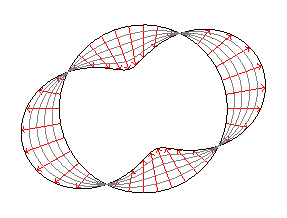
\includegraphics[width=1\linewidth]{deform_circle.pdf}}
  \caption{Deformation of the circle along a normal vector
    field.}
  \label{fig:deform-circle}
\end{figure}

\begin{figure}
  \centerline{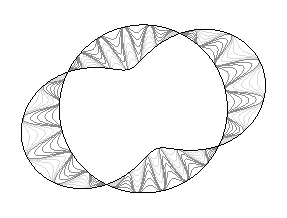
\includegraphics[width=1\linewidth]{zero_L2metric.pdf}}
  \caption{A short path in $B$.}
  \label{fig:zero_L2metric}
\end{figure}


% \hl{[This could maybe be mentioned in the beginning of the
%   construction of the tanget space?:]} We shall think of a path $\phi(t)$
% in $B$ as a smooth map \hl{(might be too restrictive)}
% \begin{equation*}
%   \phi\colon [0,1] \times \S^1 \rightarrow \R^2.
% \end{equation*}
% We have ...



\end{document}





